\begin{definition}
    For any $\mathcal{X} \in 2^\mathbb{R}$ let $\mathcal{A}(\mathcal{X})$
    be the smallest $\sigma$-algebra containing $\mathcal{X}$.
\end{definition}

\begin{lemma}
    $\mathcal{A}(\mathcal{X})$ always exists and is the intersection of all $\sigma$-algebras
    containing $\mathcal{X}$.
\end{lemma}
\begin{proof}
    We have to prove that if we intersect a bunch $\sigma$-algebras, we still get a 
    $\sigma$-algebra.
    \begin{enumerate}
        \item {
            Such an intersection is closed under complements:
            if a set belongs to the intersection of $\sigma$-algebras,
            then it belongs to each of the $\sigma$-algebras, 
            then its complement belongs to each of the $\sigma$-algebras,
            and thus its complement belongs to the intersection of 
            $\sigma$-algebras.
        }
        \item {
            In a similar way, such an intersection is closed under countable unions:
            if a number of sets all belong to the intersection of $\sigma$-algebras,
            then they all belong to each of the $\sigma$-algebras, 
            then their countable union belongs to each of the $\sigma$-algebras,
            and their countable union belongs to the intersection of 
            $\sigma$-algebras.
        }
    \end{enumerate}
\end{proof}

\begin{remark}
    We can try to construct $\mathcal{A}(\mathcal{X})$ in a different way.
    Say, $\mathcal{X}$ is not a $\sigma$-algebra. Let's enlarge it:
    first by including all the complements. Then let's enlarge it
    by all countable unions. Let's call such a set $\mathcal{X}_1$.
    But after such operation, $\mathcal{X}_1$ may be non-closed under complements.
    So we repeat such a procedure.

    And, in general: $\mathcal{X}_{n + 1}$ is obtained from $\mathcal{X}_n$
    is obtained by including into $\mathcal{X}_n$ all complements of the 
    sets from $\mathcal{X}_n$ and then including all countable unions of the obtained sets.

    \begin{figure*}[h]
        \centering
        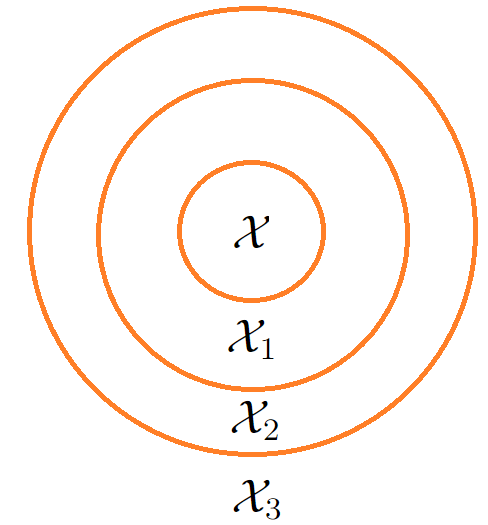
\includegraphics[width=0.3\textwidth]{some_circles}
    \end{figure*}

    It is tempting to think that $\cup_{1}^\infty \mathcal{X}_i$ is $\mathcal{A}(\mathcal{X})$.
    Is it true? No, not necessarily.
    If the sequence $\{\mathcal{X}_i\}$ eventually stabilizes, then such a construction works.
    Let's now assume that every next $\mathcal{X}_i$ is larger than the previous one.
    Then we can take $A$ from $\mathcal{X}$, $A_1$ from $\mathcal{X}_1 \setminus \mathcal{X}$,
    $A_2$ from $\mathcal{X}_2 \setminus \mathcal{X}_1$, and so on.

    Now let's look at $\cup_{1}^\infty A_i$. As a countable union, it must be contained
    in $\mathcal{A}(\mathcal{X}) = \cup_{1}^\infty \mathcal{X}_i$, thus, there exist an $n$, such that
    $\cup_{1}^\infty A_i \in \mathcal{X}_n$. But $A_{n+1} \in \mathcal{X}_{n+1} \setminus \mathcal{X}_n$?!
\end{remark}

\begin{definition}[Topological space]
    A \textit{topological space} is a set $X$ and a collection
    of subsets $O$ of $X$ (called \textit{open sets}), such that $\emptyset, X \in O$, and:
    \begin{enumerate}
        \item {
            A union of (possibly infinitely many) sets from $O$
            is in $O$.
        }
        \item {
            The intersection of finitely many sets from $O$
            is in $O$.
        }
    \end{enumerate}
    The complements of open sets are called \textit{closed sets}.
\end{definition}

\begin{definition}
    A function $f : X \to Y$ between two topological spaces is \textit{continuous} if
    the preimage of every open set is open.
\end{definition}
\begin{remark}
    It is possible to check that for $\mathbb{R}$ this definition is
    equivalent to the usual one.
\end{remark}

\begin{definition}[Borel $\sigma$-algebra]
    For a topological space $X$ its \textit{Borel $\sigma$-algebra $\mathcal{B}_X$}
    is the smallest $\sigma$-algebra on $X$ that contains all open sets. 
\end{definition}
\begin{remark}
    If it's obvious from the context which set we are talking about,
    we will just write $\mathcal{B}$ (without a subscript).
\end{remark}

\begin{theorem}
    \label{the:openMeasurable}
    $\mathcal{B}_\mathbb{R} \subset \mathcal{M}$ (all of the sets in $\mathcal{B}_\mathbb{R}$ are measurable).
\end{theorem}
\begin{proposition}
    \label{prop:bIsSmallestSigmaAlgebra}
    $\mathcal{B}$ is the smallest $\sigma$-algebra that contains all open intervals.
\end{proposition}
If we prove the proposition, the theorem will follow easily.
We know that \hyperref[prop:intervalsAreMeasurable]{all the intervals are Lebesgue-measurable}.
We know that the Lebesgue-measurable sets ($\mathcal{M}$) 
\hyperref[the:mIsSigmaAlgebra]{are a $\sigma$-algebra}.
Thus, if we take the smallest $\sigma$-algebra that contains all open intervals,
it will be a subset of $\mathcal{M}$.
\begin{proof}[Proof of Proposition~\ref{prop:bIsSmallestSigmaAlgebra}]
    We will prove that every open set $O \subset \mathbb{R}$ is a finite or
    countable union of open intervals.

    For every point $x \in O$ let $I_x$ be the largest open interval, such that
    $x \in I_x$ and $I_x \subset O$.
    It exists as a union of all such intervals. Since $O$ is open, 
    $x$ lies in $O$ with an open neighborhood,
    thus, $I_x$ is non-empty.
    \[
        \forall x \in O: x \in I_x \implies
        O = \bigcup_{x \in O} I_x
    \]
    Let's prove that $I_x \cap I_y \ne \emptyset \implies I_x = I_y$. If the intervals
    around $x$ and $y$ intersect, then $I_x \cup I_y$ is an interval as well, and
    $I_x \cup I_y \in O$ as $I_x \in O$ and $I_y \in O$. Since $I_x$ and $I_y$ are the largest such intervals, it follows that
    $I_x = I_x \cup I_y = I_y$.

    Let's say that two points $x$ and $y$ are equivalent if $I_x = I_y$.
    Since there's a lot of same intervals in $O = \cup_{x \in O} I_x$,
    we can take just a single point from every equivalence class and still get $O$ 
    as a union. Particularly, every open interval contains at least one rational point
    (as rational numbers are dense). Therefore, there's a rational point
    in every equivalence class.
    Thus,
    \[ O = \bigcup_{x \in O \cap \mathbb{Q}} I_x \]
    Since the set of rational numbers is countable, we have represented $O$
    as a countable union of open intervals, which is what we wanted.
\end{proof}

\begin{definition}
    \label{def:separable}
    A topological space is called \textit{separable}, if it contains a 
    countable dense subset.
\end{definition}
\begin{remark}
    We have proved that the Lebesgue measure exists on $\mathcal{B}_\mathbb{R}$,
    so we have a lot of measurable sets.
\end{remark}
\begin{remark}
    The Lebesgue measure can be generalized to $\mathbb{R}^n$.
\end{remark}